\documentclass[a4paper]{report}
\usepackage[utf8]{inputenc}
\usepackage[T1]{fontenc}
\usepackage{RJournal}
\usepackage{amsmath,amssymb,array}
\usepackage{booktabs}


% tightlist command for lists without linebreak
\providecommand{\tightlist}{%
  \setlength{\itemsep}{0pt}\setlength{\parskip}{0pt}}

\usepackage{longtable}

% Always define CSL refs as bib entries are contained in separate doc
% Pandoc citation processing
%From Pandoc 3.1.8
% definitions for citeproc citations
\NewDocumentCommand\citeproctext{}{}
\NewDocumentCommand\citeproc{mm}{%
  \begingroup\def\citeproctext{#2}\cite{#1}\endgroup}
\makeatletter
 % allow citations to break across lines
 \let\@cite@ofmt\@firstofone
 % avoid brackets around text for \cite:
 \def\@biblabel#1{}
 \def\@cite#1#2{{#1\if@tempswa , #2\fi}}
\makeatother
\newlength{\cslhangindent}
\setlength{\cslhangindent}{1.5em}
\newlength{\csllabelwidth}
\setlength{\csllabelwidth}{3em}
\newenvironment{CSLReferences}[2] % #1 hanging-indent, #2 entry-spacing
 {\begin{list}{}{%
  \setlength{\itemindent}{0pt}
  \setlength{\leftmargin}{0pt}
  \setlength{\parsep}{0pt}
  % turn on hanging indent if param 1 is 1
  \ifodd #1
   \setlength{\leftmargin}{\cslhangindent}
   \setlength{\itemindent}{-1\cslhangindent}
  \fi
  % set entry spacing
  \setlength{\itemsep}{#2\baselineskip}}}
 {\end{list}}
\usepackage{calc}
\newcommand{\CSLBlock}[1]{#1\hfill\break}
\newcommand{\CSLLeftMargin}[1]{\parbox[t]{\csllabelwidth}{#1}}
\newcommand{\CSLRightInline}[1]{\parbox[t]{\linewidth - \csllabelwidth}{#1}\break}
\newcommand{\CSLIndent}[1]{\hspace{\cslhangindent}#1}


\usepackage{thumbpdf,lmodern,amsfonts,amsmath,mathtools}

\begin{document}


%% do not edit, for illustration only
\sectionhead{Contributed research article}
\volume{17}
\volnumber{2}
\year{2025}
\month{June}
\setcounter{page}{146}

\begin{article}
  % !TeX root = RJwrapper.tex
\title{rqPen: An R Package for Penalized Quantile Regression}


\author{by Ben Sherwood, Shaobo Li, and Adam Maidman}

\maketitle

\abstract{%
Quantile regression directly models a conditional quantile of interest. The R package rqPen provides penalized quantile regression estimation using the lasso, elastic net, adaptive lasso, SCAD, and MCP penalties. It also provides extensions to group penalties, both for groups of predictors and grouping variable selection across quantiles. This paper presents the different approaches to penalized quantile regression and how to use the provided methods in rqPen.
}

\section{Introduction}\label{introduction}

The package \CRANpkg{rqPen} allows users to model conditional quantiles using a penalized quantile regression approach. It supports a wide range of penalties and includes cross-validation and information criterion approaches for selecting tuning parameters. \citet{origQR} proposed quantile regression as a robust alternative to mean regression that
directly models a conditional quantile of interest without the need for assumptions about the
distribution or moment conditions for the error term. Since \citet{lasso} introduced the lasso penalty, investigating the combination of different penalties and loss functions has been an active area of interest. Penalties provided in \CRANpkg{rqPen} are lasso, elastic net \citep{zou05}, SCAD \citep{fanLi}, MCP \citep{mcp}, adaptive lasso \citep{adaptiveLasso}, group lasso \citep{yuan2007}, group extensions of adaptive lasso, SCAD, and MCP \citep{grSCAD, groupReview, penBiLevel}, and a group lasso penalty where variables are grouped across quantiles \citep{heteroIdQR}. Extending the theoretical results of penalized estimators to the quantile regression setting has been an active area of research. Examples include deriving the rate of convergence for lasso \citep{qr_lasso} and group lasso \citep{qr_group_lasso} and deriving oracle properties for non-convex penalties such as SCAD and MCP \citep{lan_scad}. Discussed in these papers is how minimizing the penalized objective functions for quantile regression can be framed as linear programming problems or, in the case of group lasso, second-order cone programming problems. The linear programming formulation is particularly familiar to researchers in quantile regression because this is the most common approach for solving quantile regression problems, including in the \CRANpkg{quantreg} package \citep{crq1, crq2}, while a second-order cone programming problem can be solved using convex optimization software, including the R package \CRANpkg{Rmosek} \citep{JSSv060i05}.

The ability to analyze large data sets is one of the major appeals of penalized regression methods. However, linear programming and second-order cone programming algorithms become computationally burdensome for large data sets. Further complicating matters is that the quantile loss function is non-differentiable, while popular algorithms for penalized objective functions rely on a differentiable loss function, for instance, \citet{friedman2009glmnet} (elastic net), \citet{scadAlg} (non-convex penalties), \citet{brehenyglasso} (group non-convex penalties), and \citet{Yang2015} (group lasso). \citet{huber_cd} proposed using a Huber-type approximation of the quantile loss and coordinate descent algorithm for solving elastic net penalized quantile regression which is implemented in the R package \CRANpkg{hqreg}. Assuming a good initial estimator is provided, \citet{qr_cd} proposed a coordinate descent algorithm (QICD) for non-convex penalties. The R package \CRANpkg{conquer} approximates the quantile loss with a convolution of the quantile loss and Kernel function \citep{lowdConv, highdConv}.

The package \CRANpkg{rqPen} provides an implementation of the Huber-type approximation and linear programming algorithms. It allows users to fit quantile regression models with all of the penalty functions discussed in the first paragraph and provides tools for using cross-validation or information criterion to select tuning parameters. In addition, it provides plots for comparing cross-validation results and coefficient estimates as the sparsity parameter, \(\lambda\), changes. The package allows for estimating multiple quantiles with a call to a single function and provides plots of how coefficient values change with the different quantiles being modeled.

The packages \CRANpkg{quantreg}, \CRANpkg{conquer}, \CRANpkg{hrqglas}, and \CRANpkg{hqreg} are alternatives for penalized quantile regression in R. However, there are some substantial differences between \CRANpkg{rqPen} and these packages. The package \CRANpkg{rqPen} allows users to fit quantile regression models using the elastic net, SCAD, MCP, adaptive lasso, group lasso, group SCAD, group MCP and group adaptive lasso penalties, along with allowing users to choose between an \(L_1\) or \(L_2\) norm for all group penalties. In addition, users can fit models for multiple quantiles, use cross-validation or information criterion (IC) approaches to choose tuning parameters, and create plots of the change in coefficient estimates for different quantiles and tuning parameters. Also, commonly used functions such as \texttt{predict()}, \texttt{coef()}, and \texttt{plot()} can be used with the \texttt{rq.pen.seq} and \texttt{rq.pen.seq.cv} objects created by \CRANpkg{rqPen} functions. The package \CRANpkg{quantreg} fits unpenalized quantile regression models and provides the SCAD and lasso penalty. For both penalized and unpenalized quantile regression, \CRANpkg{conquer} offers computationally efficient estimation for large \(n\) or \(p\) data sets. Users of \CRANpkg{conquer} can choose between lasso, elastic net, group lasso, sparse-group \citep{sparseGroup}, group SCAD and group MCP. To the best of our knowledge, \CRANpkg{conquer} is the only package that offers the sparse-group lasso penalty for quantile regression. While \CRANpkg{hrqglas} provides penalized group lasso, it does not provide any of the other group penalties, nor does it allow for simultaneous estimation of multiple quantiles. Similarly, \CRANpkg{hqreg} provides the elastic net penalty using the Huber approximation, but not adaptive lasso, SCAD or MCP. However, \CRANpkg{hrqglas} and \CRANpkg{hqreg} provide methods for robust mean regression using the Huber loss function, something \CRANpkg{rqPen} does not do. Both packages are required for \CRANpkg{rqPen} and provide the backbone for the algorithms that use a Huber approximation for the group, \CRANpkg{hrqglas}, and non-group, \CRANpkg{hqreg}, penalties. The package \CRANpkg{rqPen} provides a variety of algorithms and penalty functions that users can choose from. In addition, it provides tools not available in other penalized quantile regression packages, such as plots of how coefficients change with the quantile being modeled or the sparsity parameter, allowing for multiple estimates of quantiles in a single line of code, and functions for information criterion based approaches to tuning parameter selection. Finally, it provides a penalty that guarantees consistent variable selection across quantiles, an option not available in the other packages mentioned.

\section{Penalized estimation of quantile regression}\label{penalized-estimation-of-quantile-regression}

Consider observations \(\{y_i,{\bf x}_i\}_{i=1}^n\), where \({\bf x}_i = (1,x_{i1},\ldots,x_{ip})^\top \in \mathbb{R}^{p+1}\), and the model
\begin{equation}
y_i = {\bf x}_i^\top {\boldsymbol\beta}^{\tau}_0 + \epsilon_i,
\label{eq:qrModel}
\end{equation}
where \(P(\epsilon_i < 0 | {\bf x}_i)=\tau\). Define \(\rho_\tau(u) = u[\tau-I(u<0)]\), \citet{origQR} proposed estimating \eqref{eq:qrModel} by minimizing
\begin{equation}
\sum_{i=1}^n \rho_\tau(y_i-{\bf x}_i^\top\boldsymbol \beta),
\label{eq:qr}
\end{equation}
which is available in the package \CRANpkg{quantreg}. Let \(m_i\) be the weight for observation \(i\), \(\boldsymbol w\) be a vector of weights for a predictor or group of predictors, and \(\lambda\) and \(a\) are penalty tuning parameters. The package \CRANpkg{rqPen} provides functions for estimating \(\boldsymbol \beta^\tau_0\) by minimizing
\begin{equation}
\frac{1}{n} \sum_{i=1}^n m_i \rho_\tau(y_i - {\bf x}_i^\top\boldsymbol \beta) + P_{\boldsymbol w,\lambda,a}(\boldsymbol \beta),
\label{eq:genPen}
\end{equation}
where \(\lambda>0\) and the plausible values of \(a\) depend on the penalty being used. The penalty function \(P_{\lambda,a}(\boldsymbol \beta)\) can take the form of a group or individual penalty.

\subsection{Individual Penalty}

Let \(w_j\) be a weight for a variable \(j\). For an individual penalty, \eqref{eq:genPen} has the form of
\begin{equation}
\frac{1}{n} \sum_{i=1}^n m_i \rho_\tau(y_i - {\bf x}_i^\top\boldsymbol \beta) + \sum_{j=1}^p p_{w_j\lambda,a}(|\beta_j|).
\label{eq:indPen}
\end{equation}

The package \CRANpkg{rqPen} supports four different forms of individual penalties: elastic net, adaptive lasso, SCAD and MCP. Users can also specify ridge and lasso, which are special cases of the elastic net. The SCAD, \(p^s_{\lambda,a}()\), and MCP, \(p^m_{\lambda,a}()\) penalty functions are
\begin{eqnarray*}
p^s_{\lambda,a}(|x|) &=& \lambda|x|I(0 \leq |x| < \lambda) + \frac{a\lambda|x|-(x^2+\lambda^2)/2}{a-1}I(\lambda \leq |x| \leq a\lambda) + \frac{(a+1)\lambda^2}{2}I(|x|>a\lambda),  \\
p^m_{\lambda,a}(|x|) &=& \lambda\left(|x|-\frac{x^2}{2a\lambda}\right)I(0 \leq |x| < a\lambda) + \frac{a\lambda^2}{2}I(|x|\geq a\lambda),
\end{eqnarray*}
where \(a>2\) for the SCAD penalty function and \(a>1\) for MCP.

The following defines \(P_{\lambda,a}(\boldsymbol \beta)\) for the four different penalty functions, plus two important special cases.

\begin{enumerate}
\item Elastic net: $p_{w_j\lambda,a}(|\beta_j|) = \lambda w_j \left[ \alpha |\beta_j| +  (1-\alpha) \beta_j^2 \right]$, where $a \in [0,1]$.
\begin{enumerate}
\item Lasso: a special case with $a=1$.
\item Ridge: a special case with $a=0$.
\end{enumerate}
\item Adaptive Lasso: $p_{w_j\lambda,a}(|\beta_j|) = \lambda w_j |\tilde{\beta}_j|^{-a} |\beta_j|$, where $a>0$ and $\tilde{\beta}_j$ is the Ridge estimator for the same values of $w_j$ and $\lambda$.
\item SCAD: $p_{w_j\lambda,a}(|\beta_j|) =  p^s_{w_j\lambda,a}(|\beta_j|)$, where $a>2$.
\item MCP: $p_{w_j\lambda,a}(|\beta_j|) = p^m_{w_j\lambda,a}(|\beta_j|)$, where $a>1$.
\end{enumerate}

The weights, \(w_j\), allow for different weights for predictors and must be non-negative. If \(w_j=0\) then that variable will be unpenalized. In \CRANpkg{rqPen} these weights are labeled as \texttt{penalty.factors} or \texttt{group.penalty.factors}. The lasso estimator provides the backbone for the algorithm of the three non-elastic net penalties. As \(\rho_\tau(x)+\rho_\tau(-x) = |x|\), the lasso estimator minimizes,
\begin{equation}
\frac{1}{n} \sum_{i=1}^n m_i \rho_\tau(y_i - {\bf x}_i^\top\boldsymbol \beta) +  \sum_{j=1}^p \rho_\tau(\lambda w_j\beta_j)+\rho_\tau(-\lambda w_j\beta_j).
\label{eq:lasso}
\end{equation}
For \(i \in \{1,\ldots,n\}\) define \(\tilde{y}_i = y_i\), \(\tilde{{\bf x}}_i = {\bf x}_i\), and \(\tilde{m}_i = m_i\). Let \({\bf e}_j \in \mathbb{R}^{p+1}\) represent a unit vector with a value of one in the \(j\)th position and zero in all other entries. For each \(j \in \{1,\ldots,p\}\) define \(\tilde{{\bf x}}_{n+2j-1} = -n\lambda w_j {\bf e}_j\) and \(\tilde{{\bf x}}_{n+2j} = n\lambda w_j {\bf e}_j\). In addition, for each \(i \in \{n+1,\ldots,n+2p\}\) define \(\tilde{y}_i = 0\) and \(\tilde{m}_i=1\). Then minimizing \eqref{eq:lasso} is equivalent to minimizing
\begin{equation}
\frac{1}{n} \sum_{i=1}^{n+2p} \tilde{m}_i \rho_\tau(\tilde{y}_i-\tilde{{\bf x}}_i^\top\boldsymbol \beta).
\label{eq:lassoAlt}
\end{equation}
The objective function \eqref{eq:lassoAlt} has the same form as \eqref{eq:qr} except for the scaling factor, \(n^{-1}\), and the weights. This approach of creating the augmented \(2p\) samples and then using standard quantile regression is implemented in \CRANpkg{rqPen} where the problem is solved using the \texttt{rq()} function from \CRANpkg{quantreg}. Note this approach is different from using \texttt{rq(method="lasso",...)} within \CRANpkg{quantreg}, which uses a linear programming approach but does not formulate the problem using augmented data.

For large values of \(n\) and \(p\) the linear programming algorithms become computationally burdensome. To decrease computational complexity, \citet{huber_cd} proposed approximating the quantile loss function with a Huber-like function and a new coordinate descent algorithm that requires a differentiable loss function. The Huber loss function proposed by \citet{huber1964} is
\[
h_\gamma(t) = \frac{t^2}{2\gamma}I(|t| \leq \gamma)+\left[|t|-\frac{\gamma}{2}\right]I(|t|>\gamma).
\]
Note \(\rho_\tau(u) = u[\tau-I(u<0)]=\frac{1}{2}(|u|+(2\tau-1)u)\) and for sufficiently small \(\gamma\), \(|u| \approx h_\gamma(u)\). The Huber-approximated quantile loss is
\begin{equation}
h_{\gamma}^{\tau}(u) = h_\gamma(u) + (2\tau-1)u,
\label{eq:huberQuantile}
\end{equation}
and for small \(\gamma\), \(\rho_\tau(u) \approx \frac{1}{2}h_{\gamma}^{\tau}(u)\). The package \CRANpkg{hqreg} implements the approach of \citet{huber_cd} and the function \texttt{hqreg()}, with \texttt{method="quantile"}, solves the problem of
\begin{equation}
\frac{1}{2n} \sum_{i=1}^n h_{\gamma}^{\tau}(y_i - {\bf x}_i^\top\boldsymbol \beta) +  \lambda \sum_{j=1}^p w_j|\beta_j|.
\label{eq:huberLasso}
\end{equation}

In \CRANpkg{rqPen}, solving \eqref{eq:huberLasso} is done by calling \texttt{hqreg::hqreg()} and thus \CRANpkg{hqreg} is a required package. The Huber approximation with lasso is the default for \texttt{rq.pen()}, one of the main functions in \CRANpkg{rqPen}. In addition, optimization of the adaptive lasso, SCAD and MCP problems can be solved using a version of \eqref{eq:huberLasso}, which is available in \CRANpkg{rqPen} but not \CRANpkg{hqreg}. The adaptive lasso can be solved using the same approach because it is a special case of a lasso problem with different weights for each coefficient. The initial estimators necessary for the weights are determined by a ridge estimator with the same value of \(\lambda\). The SCAD and MCP functions are approximated by a local linear approximation (LLA) as proposed by \citet{lla}. Let \(p_{w_j\lambda,a}(|\beta_j|)\) represent a generic penalty function and \(p'_{w_j\lambda,a}(|\beta_j|)\) be the derivative with respect to \(\beta_j\). Let \(\bar{\beta}_j\) be the lasso estimator for the same value of \(\lambda\) and weights. The LLA approach uses the following approximation,
\begin{align}
\frac{1}{n} \sum_{i=1}^n m_i \rho_\tau(y_i-{\bf x}_i^\top\boldsymbol \beta)  + & \sum_{j=1}^p p_{w_j\lambda,a}(|\beta_j|) \nonumber \\
 & \approx \frac{1}{n} \sum_{i=1}^n m_i \rho_\tau(y_i-{\bf x}_i^\top\boldsymbol \beta) + \sum_{j=1}^p p'_{w_j\lambda,a}(|\bar{\beta}_j|)|\beta_j|.
\label{eq:lla}
\end{align}
Again, the problem becomes a special case of a lasso estimator with specific weights for each predictor. Thus all the non-group penalties, except for elastic net and ridge, can be solved using linear programming or Huber approximation algorithms.

The elastic net penalty of
\begin{equation}
\frac{1}{n} \sum_{i=1}^n m_i \rho_\tau(y_i - {\bf x}_i^\top\boldsymbol \beta) + \lambda \sum_{j=1}^p w_j \left[ a|\beta_j|+(1-a)\beta_j^2\right],
\label{eq:enet}
\end{equation}
cannot be framed as a linear programming problem because of the ridge penalty. Thus for \(a \neq 1\), the \CRANpkg{rqPen} implementation of elastic net only uses the Huber approximation approach provided in \CRANpkg{hqreg}. While \CRANpkg{hqreg} provides a computational backbone, \CRANpkg{rqPen} provides SCAD, MCP, and adaptive lasso penalties that are not provided in \texttt{hqreg()}. In addition, \texttt{hqreg()} does not include any group penalties or allow for weights for observations, \(m_i\). If weights are specified then the group lasso with singleton groups, implemented in \CRANpkg{hrqglas}, is used instead of using \texttt{hqreg()} from \CRANpkg{hqreg}.

\subsection{Group Penalty predictors}\label{group-penalty-predictors}

When there exists a group structure to the predictors then a group penalty can often account for this structure. For instance, non-binary categorical variables or polynomial transformations of predictors. This section assumes the \(p\) predictors are partitioned into \(G\) groups and \(\boldsymbol \beta_g\) represents the coefficients associated with the \(g\)th group of predictors. Group penalized quantile regression estimators minimize
\begin{equation}
\frac{1}{n} \sum_{i=1}^n m_i \rho_\tau(y_i - {\bf x}_i^\top\boldsymbol \beta) + \sum_{g=1}^G p_{w_g\lambda,a}(||\boldsymbol \beta_g||_q).
\label{eq:groupForm}
\end{equation}

Users can choose four penalty functions for \(p_{w_g,\lambda,a}()\): (1) lasso; (2) Adaptive lasso; (3) SCAD; and (4) MCP. Specifically,

\begin{enumerate}
\item lasso: $\sum_{g=1}^G p_{w_g\lambda,a}(||\boldsymbol \beta_g||_2)=\lambda \sum_{g=1}^G w_g ||\boldsymbol \beta_g||_2$;
\item Adaptive lasso: $\sum_{g=1}^G p_{w_g\lambda,a}(||\boldsymbol \beta_g||_q)= \lambda \sum_{g=1}^G w_g ||\tilde{\boldsymbol \beta}_g||_q^{-a} ||\boldsymbol \beta_g||_q$, where $a>0$ and $\tilde{\beta}_j$ is the Ridge estimator for the same values of $\lambda$ and $w_g$;
\item SCAD: $P_a(\boldsymbol \beta) = \sum_{g=1}^G p^s_{w_g\lambda,a}(||\boldsymbol \beta_g||_q)$, where $a>2$;
\item MCP: $P_a(\boldsymbol \beta) = \sum_{g=1}^G p^m_{w_g\lambda,a}(||\boldsymbol \beta_g||_q)$, where $a>1$.
\end{enumerate}

The values of \(q\) in \texttt{rq.group.pen()} is limited to \(q \in \{1,2\}\) and can be changed with \texttt{norm=q}. If \(q=2\) then group variable selection will be all-or-nothing, that is all variables within a group will be selected or none of them will be. The choice of \(q=1\) allows for bi-level variable selection \citep{penBiLevel}. Users cannot specify \texttt{norm=1} and \texttt{penalty="gLASSO"}, default penalty of group lasso, because that is equivalent to the individual lasso penalty implemented in \texttt{rq.pen()}.

\citet{groupReview} provide an excellent review of group penalties, including a discussion of the use of \(q=1\). For differentiable loss functions, \citet{penBiLevel} provide a computational perspective on \(q=1\), while \citet{mestatp} compare oracle model selection properties for \(q=1\) and \(q=2\).

For \(q=1\), the group lasso estimator becomes a special case of the individual lasso estimator, and this is also true for the adaptive lasso penalty. For the SCAD and MCP penalties, LLA will be used to approximate the non-convex penalties. Let \(\bar{\boldsymbol \beta}_g\) be an initial group lasso estimator and the penalized objective function is approximated by
\begin{equation}
\frac{1}{n} \sum_{i=1}^n m_i \rho_\tau(y_i - {\bf x}_i^\top\boldsymbol \beta) + \sum_{g=1}^G p'_{w_g\lambda,a}(||\bar{\boldsymbol \beta}_g||_q)||\boldsymbol \beta_g||_q.
\label{eq:groupFormlla}
\end{equation}

Thus for the case of \(q=1\) this becomes an individual lasso problem and the algorithms discussed in the previous section apply. In particular, the problem can be framed as a linear programming problem. While for \(q=2\) \eqref{eq:groupFormlla} becomes a special case of the group lasso problem. These group lasso problems are not linear programming problems, but second-order cone programming problems. Second-order cone programming problems can be solved by existing convex optimization software such as \CRANpkg{Rmosek} \citep{JSSv060i05}. However, there are some barriers to using \CRANpkg{Rmosek}, for instance it requires a copy of Mosek installed on the user's computer. In addition, similar to linear programming problems, second-order cone programming algorithms can be computationally burdensome for large values of \(n\) or \(p\). For \(q=2\), the Huber approximation described in the previous subsection is used. However, \CRANpkg{hqreg} cannot be used to solve this problem because the approach of \citet{huber_cd} is not for a group penalty. Instead, the algorithm of \citet{Yang2015} is implemented. See \citet{SherwoodLi2022} for details regarding the application of this algorithm to the asymmetric Huber regression setting. This approach is available in the package \CRANpkg{hrqglas}, which is maintained by two of the authors and provides the computational backbone for the \(L_2\) group penalties.

\subsection{Estimation of Multiple Quantiles}\label{estimation-of-multiple-quantiles}

For a set of quantiles of interest, \((\tau_1,\ldots,\tau_B)\), \citet{qr_lasso} proposed minimizing,
\begin{equation}
\frac{1}{n} \sum_{b=1}^B\sum_{i=1}^n m_i \rho_{\tau_b}\left(y_i - {\bf x}_i^\top\boldsymbol \beta^{\tau_b}\right) + \frac{\tilde{\lambda}}{n} \sum_{b=1}^B\sum_{j=1}^p \sqrt{\tau_b(1-\tau_b)} \hat{\sigma}_j |\beta^{\tau_b}_j|,
\label{eq:qrBel}
\end{equation}
where \(\hat{\sigma}_j = n^{-1}\sum_{i=1}^n x_{ij}^2\). We use \(\tilde{\lambda}\) in \eqref{eq:qrBel} to emphasize that the scaling of the tuning parameter is different than that used in \CRANpkg{rqPen}, specifically \(\lambda=\frac{\tilde{\lambda}}{n}\). The penalized objective function of \eqref{eq:qrBel} provides a quantile specific weight of \(\sqrt{\tau_b(1-\tau_b)}\) and a predictor specific weight of \(\hat{\sigma}_j\), while \(\lambda\) is assumed to have the same value. In \CRANpkg{rqPen}, this approach is generalized to allow for different penalties and user choices of the quantile, predictor, and observation weights. For an individual penalty the estimator minimizes,
\begin{equation}
\frac{1}{n} \sum_{b=1}^B\sum_{i=1}^n m_i \rho_{\tau_b}\left(y_i - {\bf x}_i^\top\boldsymbol \beta^{\tau_b}\right) + \sum_{b=1}^B\sum_{j=1}^p p_{w_jd_b\lambda,a}(|\beta^{\tau_b}_j|).
\label{eq:multtau}
\end{equation}
For a group penalty the penalized objective function is
\begin{equation}
\frac{1}{n} \sum_{b=1}^B \sum_{i=1}^n m_i \rho_{\tau_b}\left(y_i - {\bf x}_i^\top\boldsymbol \beta^{\tau_b}\right) + \sum_{b=1}^B \sum_{g=1}^G p_{w_gd_b\lambda,a}(||\boldsymbol \beta_g||_q).
\label{eq:multtaug}
\end{equation}
Note, the \(w_jd_b\lambda\) term allows users to specify specific weights for a predictor, \(w_j\), and specific weights for a quantile, \(d_b\). For instance, if a user chooses the lasso penalty with \(w_j=n^{-1}\sum_{i=1}^nx_{ij}^2\), \(d_b=n^{-1}\sqrt{\tau_b(1-\tau_b)}\), and \(m_i=1\) then \eqref{eq:multtau} is equivalent to \eqref{eq:qrBel}. The optimization of \eqref{eq:multtau} and \eqref{eq:multtaug} consist of \(B\) different optimization problems. In \CRANpkg{rqPen} they are solved separately using the algorithms that have been discussed previously, except the same sequence of \(\lambda\) is used for all \(B\) problems. In \citet{qr_lasso} they suggest choosing the same value of \(\lambda\) for all the quantiles, albeit with the quantile-specific weights. We later present how users can choose a single value of \(\lambda\) and coefficient estimates come from either \eqref{eq:multtau} or \eqref{eq:multtaug}. Alternatively, users can choose \(B\) different values of \(\lambda\) and then the solutions come from \(B\) different optimizations of \eqref{eq:indPen} or \eqref{eq:groupForm}. The latter approach is equivalent to a data-driven approach for estimating the optimal quantile-specific weights, \(d_b\).

\subsubsection{Consistent selection across quantiles}\label{consistent-selection-across-quantiles}

The penalties discussed previously do not ensure consistent selection across the quantiles. That is for two quantiles \(\tau_1\) and \(\tau_2\), it is possible for a variable's coefficient to be non-zero at \(\tau_1\), but zero at \(\tau_2\). Our opinion is this is often hard to interpret. Consider the case where \(B\) quantiles are considered. Define, \(\boldsymbol \beta^j = (\beta_{j}^{\tau_1},\ldots,\beta^{\tau_B}_j)^\top \in \mathbb{R}^{B}\) as the vector of the \(j\)th coefficient for all \(B\) quantiles. Define \(||\boldsymbol \beta^j||_{2,\boldsymbol w,\boldsymbol d}=\sqrt{\sum_{b=1}^B d_b w_j (\beta^{\tau_b}_{j})^2}\), as weighted \(L_2\)-norm that allows for predictor, \(m_j\), and quantile, \(w_k\), specific weights. If a user desires consistent variable selection across quantiles they can use the group quantile penalized objective function,
\begin{equation}
\frac{1}{n} \sum_{b=1}^B \sum_{i=1}^n m_i \rho_{\tau_b}\left(y_i - {\bf x}_i^\top\boldsymbol \beta^{\tau_b}\right) + \lambda \sum_{j=1}^p ||\boldsymbol \beta^j||_{2,\boldsymbol w,\boldsymbol d}.
\label{eq:gql}
\end{equation}

We refer to this penalty as the group quantile penalty \citep{gqlasso}.

\subsection{Tuning parameter selection}\label{tuning-parameter-selection}

There are two tuning parameters, \(\lambda\) and \(a\), that need to be set. The value of \(a\) defaults to commonly used values for each penalty: (1) elastic-net (\(a=1\)); (2) adaptive lasso (\(a=1\)); (3) SCAD (\(a=3.7\)); and (4) MCP (\(a=3\)). Users can also specify values of \(a\), except for the cases of Ridge (\(a=0\)) and lasso (\(a=1\)) where the value of \(a\) is fixed. Typically the value of \(a\) is not as much of a concern as the value of \(\lambda\), a potential notable exception to this would be the elastic net penalty. Users can specify a sequence for values of \(\lambda\) otherwise, a sequence will be automatically generated. Define \(H_\gamma^\tau(\boldsymbol \beta) = \frac{1}{2n} \sum_{i=1}^n m_i h_\gamma^\tau(y_i - {\bf x}_i^\top\boldsymbol \beta)\). Define \(\tilde{a}=a\) if the elastic net penalty is used and one otherwise. If \(a=0\), that is the ridge penalty is being used, then \(\tilde{a}=.001\). The default value for an individual penalty is \(\lambda_{\max} = \max_{j,b} 1.05\left|\frac{\partial}{\partial \beta_j} H_\gamma^{\tau_b}(\mathbf{0}_{p+1})\right|(w_jd_b\tilde{a})^{-1}\) and for a group penalty is \(\lambda_{\max} = \max_{g,b} 1.05\left|\left| \frac{\partial}{\partial \boldsymbol \beta_g} H_\gamma^{\tau_b}(\mathbf{0}_{p+1})\right|\right|_q (w_gd_b)^{-1}\). The 1.05 multiplier is used to ensure that \(\lambda_{\max}\) provides a completely sparse solution regardless of whether the Huber approximation is used or not. If any predictors or groups are unpenalized at a given quantile then they are excluded from these calculations.

Both cross-validation and information criterion are provided as tools for selecting the optimal pair of \((\lambda,a)\). Let \(\hat{\boldsymbol \beta}^\tau_{\lambda,a}\) be the coefficient estimates for quantile \(\tau\) using tuning parameters \(\lambda\) and \(a\). Define \(k^\tau_{\lambda,a}\) as the number of non-zero coefficients in \(\hat{\beta}_{\lambda,a}^\tau\). The quantile information criterion (QIC) is defined as
\begin{equation}
QIC(\tau,\lambda,a) = \log\left[ \sum_{i=1}^n m_i \rho_\tau(y_i-{\bf x}_i^\top \hat{\boldsymbol \beta}^\tau_{\lambda,a}) \right] + \frac{mk^\tau_{\lambda,a}}{2n},
\label{eq:qic}
\end{equation}
where the value of \(m\) depends on the criterion being used. Users can select between AIC (\(m=2\)), BIC {[}\(m=\log(n)\){]}, and a version of the large \(p\) BIC proposed by \citet[\(m=\log(n)\log(p)\)]{qrbic}.

Cross-validation is the other approach implemented for choosing the optimal pair of \((\lambda,a)\). Consider the case of \(K\) folds, let \(n_k\) be the number of observations in the \(k\)th fold, \(y_i^k\), \({\bf x}_i^k\), and \(m_i^k\) be the \(i\)th response, predictor vector, and weights for the \(k\)th fold and \(\hat{\boldsymbol \beta}^{\tau_b}_{-k,\lambda,a}\) be the fit for the \(b\)th quantile excluding the \(k\)th fold for given values of \(\lambda\) and \(a\). By default, even if Huber approximations are used, cross-validation is done using quantile loss. However, this can be changed by setting \texttt{cvFunc} in the later described functions \texttt{rq.group.pen.cv()}, \texttt{rq.gq.pen.cv()}, or \texttt{rq.pen.cv()}. For instance, \texttt{cvFunc=abs} will use absolute value loss regardless of the quantile being modeled. For simplicity of presentation, the following assumes quantile loss is used. The average quantile loss at a given fold is
\begin{equation}
C_k^\tau(\lambda,a) = \frac{1}{n_k} \sum_{i=1}^{n_k} m_i^k \rho_\tau(y_i^k-{{\bf x}_i^k}^\top\hat{\boldsymbol \beta}^{\tau}_{-k,\lambda,a}).
\label{eq:cv1}
\end{equation}
The cross-validation functions return two summaries of the cross-validation for selecting \((\lambda,a)\). The return value \texttt{btr} provides a table of the values of \(a\) and \(\lambda\) that minimize
\begin{equation}
C^\tau(\lambda,a) = \frac{1}{K} \sum_{k=1}^K C_k^\tau(\lambda,a).
\label{eq:cv2}
\end{equation}
In addition it provides the \(\lambda\) value associated with the sparsest solution that is within one standard error of the value that minimizes \eqref{eq:cv2}. The standard error for a given pair of \((\lambda,a)\) is calculated as
\begin{equation}
\sqrt{\frac{1}{K-1} \sum_{k=1}^K \left[C_k^\tau(\lambda,a)-C^\tau(\lambda,a) \right]^2}.
\end{equation}
The average summary can be replaced by changing the parameter \texttt{cvSummary}. For instance, \texttt{cvSummary=median} would use the median values of \(C_k^\tau(\lambda,a)\).

Users can also choose to optimize \(\lambda\) and \(a\), so they are the same values across all quantiles. When evaluating the cross-validation error they can choose to not provide equal weight to each quantile by entering quantile specific weights of \(z_b\). The return value \texttt{gtr} provides results for the value of \(\lambda\) and \(a\) that minimize
\begin{equation}
C(\lambda,a) = \sum_{b=1}^B z_b C^{\tau_b}(\lambda,a).
\label{eq:cv3}
\end{equation}
Users can choose between a single pair of \((\lambda,a)\) that minimizes \eqref{eq:cv3} or \(B\), potentially different, pairs that minimize \eqref{eq:cv2} separately for each quantile except for when minimizing \eqref{eq:gql}. That is a joint optimization problem and thus only joint selection of tuning parameters using \eqref{eq:cv3} is allowed. In addition, results for the one standard error approach, where the standard error for a fixed \((\lambda,a)\) pair is
\begin{equation}
\sqrt{\frac{1}{K-1}\sum_{k=1}^K \sum_{b=1}^B z_b \left[C_k^\tau(\lambda,a) -C^\tau(\lambda,a) \right]^2},
\end{equation}
are provided. The one standard error rule finds the sparsest solution, by increasing \(\lambda\), where the value of \eqref{eq:cv2} or \eqref{eq:cv3} are within one standard error of the optimal value, assuming the optimal \(a\) is fixed.

By setting \texttt{groupError=FALSE} each observation is weighted equally and \eqref{eq:cv2} and \eqref{eq:cv3} are replaced by \(\sum_{k=1}^K n_k C_k^\tau(\lambda,a)\),
and \(\sum_{b=1}^B z_b \sum_{k=1}^K n_k C_k^\tau(\lambda,a)\), respectively.

\subsubsection{Tuning parameter selection for multiple quantiles using an information criterion}\label{tuning-parameter-selection-for-multiple-quantiles-using-an-information-criterion}

For the case of multiple, \(B\), quantiles being modeled, \CRANpkg{rqPen} offers two different approaches for selecting the tuning parameters. One approach is to select \(B\) pairs of \((\lambda,a)\) that minimize the \(B\) different versions of \eqref{eq:qic}. The other approach is given weights \((z_1,\ldots,z_b)\), the optimal pair of \((\lambda,a)\) minimizes,
\begin{equation}
\sum_{b=1}^B z_b QIC(\tau_b,\lambda,a).
\label{eq:jointQic}
\end{equation}
The weights offer flexibility to a user who wants to provide more weight to a specific quantile. The default value for all the weights is one thus giving equal weight to each quantile.

\subsection{Additional notes on Huber approximation}\label{additional-notes-on-huber-approximation}

For Huber approximation, a value of \(\gamma\) is needed. If \(\gamma\) is too large then the estimator will have a large amount of bias. If \(\gamma\) is too small the algorithms will become unstable. The values of \(\gamma\) are updated for each value of \(\lambda\). Let \({\bf r}^k\) be the vector of residuals corresponding to the estimator using the \(k\)th value of \(\lambda\), \(\lambda^k\), and \(Q_{.1}(|{\bf r}^k|)\) be the 10th percentile of the absolute values of these residuals. For an individual penalty we use what is implemented in \CRANpkg{hqreg}, which is very similar to what is outlined by \citet{huber_cd}. Specifically,
\begin{eqnarray*}
\gamma^k &=& I(|1-\tau|< .05)\max\left\{.0001,\min\left[\gamma^{k-1},Q_{.01}(|{\bf r}^k|)\right]\right\} \\
&& + I(|1-\tau|>=.05)\max\left\{.001,\min\left[\gamma^{k-1},Q_{.1}(|{\bf r}^k|)\right]\right\}.
\end{eqnarray*}

For the group penalties, as presented in \citet{SherwoodLi2022},
\begin{equation*}
\gamma^k = \min\left\{4, \max\left[.001, Q_{.1}(|{\bf r}^k|) \right] \right\}.
\end{equation*}

One reason the linear and second-order cone programming problems are computationally slow for larger values of \(p\) is they optimize across all potential predictors. \citet{tibshirani2012strong} proposed a strong rule for discarding predictors that can greatly decrease the computational complexity of penalized optimization. The strong rule assumes a differentiable loss function and thus is only implemented for the Huber approximations. In addition, the Huber approximation approaches use warm starts across a path of potential \(\lambda\) values. It starts with the largest potential value of \(\lambda\) then uses that solution as the initial value for the next largest potential value of \(\lambda\). This iterative process is continued until all solutions have been found. The linear programming approaches rely on \texttt{quantreg::rq()} which does not have an option for initial values. Thus warm starts are not implemented for those approaches. For an individual penalty, the calculations of the strong rule are done in the package \CRANpkg{hqreg}, and details can be found in \citet{huber_cd}. A similar approach has been used for group penalties \citep{SherwoodLi2022}.

\section{Description of functions}\label{description-of-functions}

Below are the main functions of \CRANpkg{rqPen} and an S3 method that is unique to \CRANpkg{rqPen}, \texttt{bytau.plot()}.

\begin{itemize}
\tightlist
\item
  \texttt{rq.pen()} minimizes \eqref{eq:multtau} to provide estimates of a quantile regression model, for potentially multiple quantiles, using an individual penalty of either elastic-net, adaptive lasso, SCAD, or MCP. If not specified, a sequence of \(\lambda\) values is automatically generated. Returns an \texttt{rq.pen.seq} S3 object that works with \texttt{bytau.plot()}, \texttt{coef()}, \texttt{plot()}, \texttt{predict()}, and \texttt{print()} methods.
\item
  \texttt{rq.gq.pen()} minimizes \eqref{eq:gql} to provide a quantile regression model for multiple quantiles using the group quantile lasso penalty. It also returns an \texttt{rq.pen.seq} S3 object and can be used with the same methods listed above.
\item
  \texttt{rq.group.pen()} minimizes \eqref{eq:multtaug} and is a group penalty version of \texttt{rq.pen()}. Users have access to group versions of the lasso, adaptive lasso, SCAD, and MCP penalties. The lasso penalty is restricted to the L2-norm. For other penalties, users can choose between the L1- or L2-norm. It also returns an \texttt{rq.pen.seq} S3 object and can be used with the same methods listed above.
\item
  \texttt{rq.pen.cv()} automates K-folds cross-validation for selecting the tuning parameters \(\lambda\) and \(a\). If \(\lambda\) is left undefined, a sequence of \(\lambda\) values will be automatically generated. For \(a\), the default values described earlier will be used, unless the user specifies a sequence. If multiple quantiles are modeled then it provides the optimal pair of \((\lambda,a)\) for each quantile and the optimal pair across all quantiles. Returns an \texttt{rq.pen.seq.cv} S3 object that works with \texttt{bytau.plot()}, \texttt{coef()}, \texttt{plot()}, \texttt{predict()}, and \texttt{print()} methods.
\item
  \texttt{rq.gq.pen.cv()} is the group quantile lasso version of \texttt{rq.pen.cv()}. It does everything listed above, but for the group quantile penalty. It also returns an \texttt{rq.pen.seq.cv} object.
\item
  \texttt{rq.group.pen.cv()} is the group version of \texttt{rq.pen.cv()}. It does everything listed above, but for group penalties. It also returns an \texttt{rq.pen.seq.cv} object.
\item
  \texttt{qic.select()} takes an \texttt{rq.pen.seq} or \texttt{rq.pen.seq.cv} object and provides the optimal values of \((\lambda,a)\) using an information criterion, as explained in the previous section. It returns a `\texttt{qic.select}' S3 object that works with \texttt{coef()}, \texttt{predict()}, and \texttt{print()} methods.
\item
  \texttt{bytau.plot()} plots coefficient estimates for each predictor as a function of \(\tau\).
\end{itemize}

The \texttt{rq.pen()} function provides estimates of conditional quantiles from minimizing a penalized objective function for a sequence of \(\lambda\) values.

\begin{verbatim}
rq.pen(x, y, tau = 0.5, lambda = NULL,
        penalty = c("LASSO", "Ridge", "ENet", "aLASSO", "SCAD", "MCP"),
        a = NULL, nlambda = 100, eps = ifelse(nrow(x) < ncol(x), 0.05, 0.01),
        penalty.factor = rep(1, ncol(x)),
        alg = ifelse(sum(dim(x)) < 200, "br", "huber"), scalex = TRUE,
        tau.penalty.factor = rep(1, length(tau)),
        coef.cutoff = 1e-08, max.iter = 10000, converge.eps = 1e-07,
        lambda.discard = TRUE, weights=NULL, ...)
\end{verbatim}

The function \texttt{rq.pen()} requires a design matrix \texttt{x} and vector of response \texttt{y}. The predictors in the design matrix will be centered to have mean zero and standard deviation one when minimizing the penalized objective function unless \texttt{scalex} is set to FALSE. While the predictors are scaled, the coefficients are returned on the original scale of \texttt{x}. The quantiles modeled are set with \texttt{tau}. Users can choose the \texttt{penalty} function, with the default being lasso. A pre-specified lambda sequence can be set, \texttt{lambda}. If the user does not specify a sequence of \(\lambda\) values then \(\lambda_{min}=\epsilon\lambda_{max}\), where \(\epsilon\) can be set by \texttt{eps} and \texttt{nlambda} is the number of \(\lambda\) values considered. Though very small values of \(\lambda\) may be discarded if the coefficient estimates are not changing much with smaller values of \(\lambda\), unless \texttt{lambda.discard=FALSE}. For non-ridge or non-lasso penalties, a sequence of values can also be selected for \texttt{a}. If \texttt{a} is not set then default values depend on the penalty, elastic-net (\(a=0\)), adaptive lasso (\(a=1\)), SCAD (\(a=3.7\)) and MCP (\(a=3\)). Penalty factors can be set for predictors, \texttt{penalty.factor}, or quantiles, \texttt{tau.penalty.factor}. Observation weights are set using \texttt{weights}. The linear programming algorithms can provide very small, but non-zero estimates, and these coefficients are set to zero if they are below \texttt{coef.cutoff}. The choice of algorithm can be set using \texttt{alg}. Two linear programming algorithms are provided, the Barrodale and Roberts algorithm (br) \citep{br}, as described in \citet{crq1} and \citet{crq2}, and the Frisch-Newton (fn) approach, described in \citet{portnoy1997}. Both approaches rely on implementations in \CRANpkg{quantreg}. Setting \texttt{rq.pen(alg="huber")} uses the approach of \citet{huber_cd} implemented in \CRANpkg{hqreg}. In addition, they can set the maximum number of iterations, \texttt{max.iter}, or convergence criteria, \texttt{converge.eps}, though these only apply to the ``huber'\,' algorithms.

\begin{verbatim}
coef.rq.pen.seq(object, tau = NULL, a = NULL, lambda = NULL, modelsIndex = NULL,
    lambdaIndex = NULL, ...)
\end{verbatim}

Using \texttt{coef()}, users can extract coefficients for specific quantiles, \texttt{tau}, and tuning parameters, \texttt{a} and \texttt{lambda}, from class \texttt{rq.pen.seq} object. Alternatively, they can directly specify the models and lambda values using \texttt{modelsIndex} and \texttt{lambdaIndex}, respectively. If none of these values are set then a matrix of coefficients for all quantiles and tuning parameters will be returned. \newline

\begin{verbatim}
coef.rq.pen.seq.cv(object, septau = TRUE, cvmin = TRUE, useDefaults = TRUE,
    tau = NULL, ...)
\end{verbatim}

With an \texttt{rq.pen.seq.cv} object, the \texttt{coef()} function returns coefficients based on the cross-validation results. If \texttt{cvmin=TRUE} then the tuning parameters associated with the minimum cross-validation error are returned, otherwise the one standard error rule is used. When \texttt{septau=TRUE} then the tuning parameters are optimized individually for each quantile. Users can identify the specific quantiles, \texttt{tau}, they wish to return. The default is to return results for all quantiles. Setting \texttt{useDefaults=FALSE} ignores the cross-validation results and users can use the arguments in \texttt{coef.rq.pen.seq()} to select coefficients. For instance, if \texttt{useDefaults=FALSE} and no other arguments are provided then all coefficients are returned.

Function \texttt{bytau.plot()} has a similar form for the \texttt{rq.pen.seq} and \texttt{rq.pen.seq.cv} objects. \newline

\begin{verbatim}
bytau.plot.rq.pen.seq(x, a = NULL, lambda = NULL, lambdaIndex = NULL, ...)
\end{verbatim}

\begin{verbatim}
bytau.plot.rq.pen.seq.cv(x, septau = TRUE, cvmin = TRUE, useDefaults = TRUE, ...)
\end{verbatim}

These functions produce a plot of how coefficients change with quantiles. The arguments in \texttt{bytau.plot.rq.pen.seq()} and \texttt{bytau.plot.rq.pen.seq.cv()} are the same as those covered for \texttt{coef()}, but with one major difference. Only one vector of coefficients can be provided for each quantile. When using an \texttt{rq.pen.seq} object, users must specify a single pair of \((\lambda,a)\). When using an \texttt{rq.pen.seq.cv} object, users can rely on the default tools for selecting coefficients or specify a single pair of \(\lambda\) and \(a\).

Both \texttt{rq.pen.seq} and \texttt{rq.pen.seq.cv} objects have \texttt{plot()} functions. Using \texttt{plot()} with an \texttt{rq.pen.seq.cv} object provides a plot of how the cross-validation error changes with \(\lambda\) for each quantile.

\begin{verbatim}
plot.rq.pen.seq.cv(x, septau = TRUE, tau = NULL, logLambda = FALSE, main = NULL, ...)
\end{verbatim}

If \texttt{septau=TRUE} then a separate plot is created for each quantile, otherwise one plot is created that combines the cross-validation error across all quantiles. Users can limit the plots to a subset of quantiles, \texttt{tau}. If \texttt{logLambda=TRUE} then the x-axis will be \(\log(\lambda)\). The \texttt{main} text can be set otherwise the main title depends on the name of the variable and the value of \texttt{septau}.

While \texttt{plot()} for an \texttt{rq.pen.seq} object creates a plot of the coefficients as they change with \(\lambda\).

\begin{verbatim}
plot.rq.pen.seq(x, vars = NULL, logLambda = TRUE, tau = NULL, a = NULL,
    lambda = NULL, modelsIndex = NULL, lambdaIndex = NULL, main = NULL, ...)
\end{verbatim}

The \texttt{plot()} function will create a plot for each combination of \(\tau\) and \(a\). Users can specify specific values of \texttt{tau} and \texttt{a} if they only want to consider a subset. They can also limit the values of \texttt{lambda}. Choice of models and \(\lambda\) values can also be done using \texttt{modelsIndex} and \texttt{lambdaIndex}. The \texttt{main} text can be set. If \texttt{logLambda=TRUE} then the \(\lambda\) values are reported on the natural log scale.

\section{Applications}\label{applications}

This section details how to use individual and group penalties. Different individual penalties and algorithms will be applied to the Barro data set from the \CRANpkg{quantreg} package. In addition, the group quantile penalty is used with the Barro data set. While the group penalties for predictors will be used with the Ames housing data \citep{de2011ames} available in \CRANpkg{AmesHousing}.

\subsection{The Barro data set}\label{the-barro-data-set}

The Barro data set, available in \CRANpkg{quantreg}, contains GDP growth rates and 13 other potential explanatory variables. See \citet{barro} for more details.

\subsubsection{Using different algorithms}\label{using-different-algorithms}

First, we look at fitting a model with the SCAD penalty for \(\tau=.5\) using three different algorithms.

\begin{verbatim}
library(rqPen)
#quantreg is required for rqPen, but call directly here
#because we need the Barro data set
library(quantreg)
data(barro)
y <- barro$y.net
x <- as.matrix(barro[,-1])
qbr <- rq.pen(x,y,alg="br", penalty="SCAD")
qfn <- rq.pen(x,y,alg="fn", penalty="SCAD")
qhuber <- rq.pen(x,y,alg="huber",penalty="SCAD")
\end{verbatim}

Where ``br'' and ``fn'' are the Barrodale and Roberts \citep{crq1, crq2} and Frisch-Newton \citep{portnoy1997} interior point method for linear programming problems implemented in \texttt{quantreg::rq()}. The following code takes the 25th value in the sequence of \(\lambda\) values and compares the coefficients for the three different approaches creating three different \texttt{rq.pen.seq} objects.

\begin{verbatim}
targetLambda <- qbr$lambda[25]
brCoef <- coefficients(qbr,lambda=targetLambda)
fnCoef <- coefficients(qfn, lambda=targetLambda)
huberCoef <- coefficients(qhuber, lambda=targetLambda)
coefDf <- cbind(brCoef,fnCoef,huberCoef)
colnames(coefDf) <- c("br","fn","huber")
coefDf
\end{verbatim}

\begin{verbatim}
#>                    br          fn       huber
#> intercept  0.02018841  0.02018852  0.02131606
#> lgdp2      0.00000000  0.00000000  0.00000000
#> mse2       0.00000000  0.00000000  0.00000000
#> fse2       0.00000000  0.00000000  0.00000000
#> fhe2       0.00000000  0.00000000  0.00000000
#> mhe2       0.00000000  0.00000000  0.00000000
#> lexp2      0.00000000  0.00000000  0.00000000
#> lintr2     0.00000000  0.00000000  0.00000000
#> gedy2     -0.01773640 -0.01773726 -0.06602351
#> Iy2        0.02366121  0.02366100  0.02917322
#> gcony2    -0.02007166 -0.02007206 -0.02269923
#> lblakp2   -0.01433958 -0.01433962 -0.01524323
#> pol2      -0.01112295 -0.01112292 -0.01067910
#> ttrad2     0.04986245  0.04986267  0.04863867
\end{verbatim}

The three different algorithms provide coefficient estimates that are different but similar. For larger data sets, with a large number of observations or variables, we recommend using the Huber approximation because this greatly reduces computational time while providing a reasonable solution \citep{huber_cd}. The following presents a plot of how the coefficient values from \texttt{qhuber} change with \(\lambda\).

\begin{verbatim}
plot(qhuber)
\end{verbatim}

\begin{center}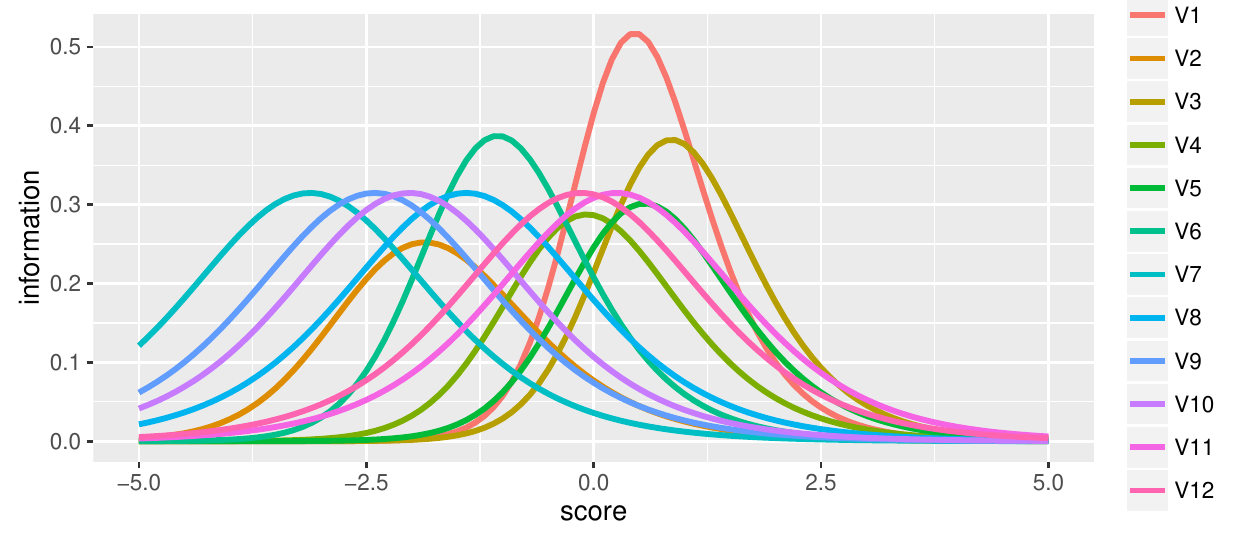
\includegraphics[width=1\linewidth]{RJ-2025-017_files/figure-latex/unnamed-chunk-10-1} \end{center}

\subsubsection{Multiple quantiles}\label{multiple-quantiles}

Next, we fit a model for multiple quantiles of \(\tau \in \{.1,.5,.9\}\) and will also consider values of \(a \in \{3,4\}\) for the additional tuning parameter for SCAD. A fit with multiple quantiles remains an \texttt{rq.pen.seq} object.

\begin{verbatim}
qmult <- rq.pen(x,y,tau=c(.1,.5,.9),a=c(3,4),penalty="SCAD")
\end{verbatim}

The following code provides a plot of the coefficients for \(\tau=.1\) and \(a=4\).

\begin{verbatim}
plot(qmult, tau=.1,a=4)
\end{verbatim}

\begin{center}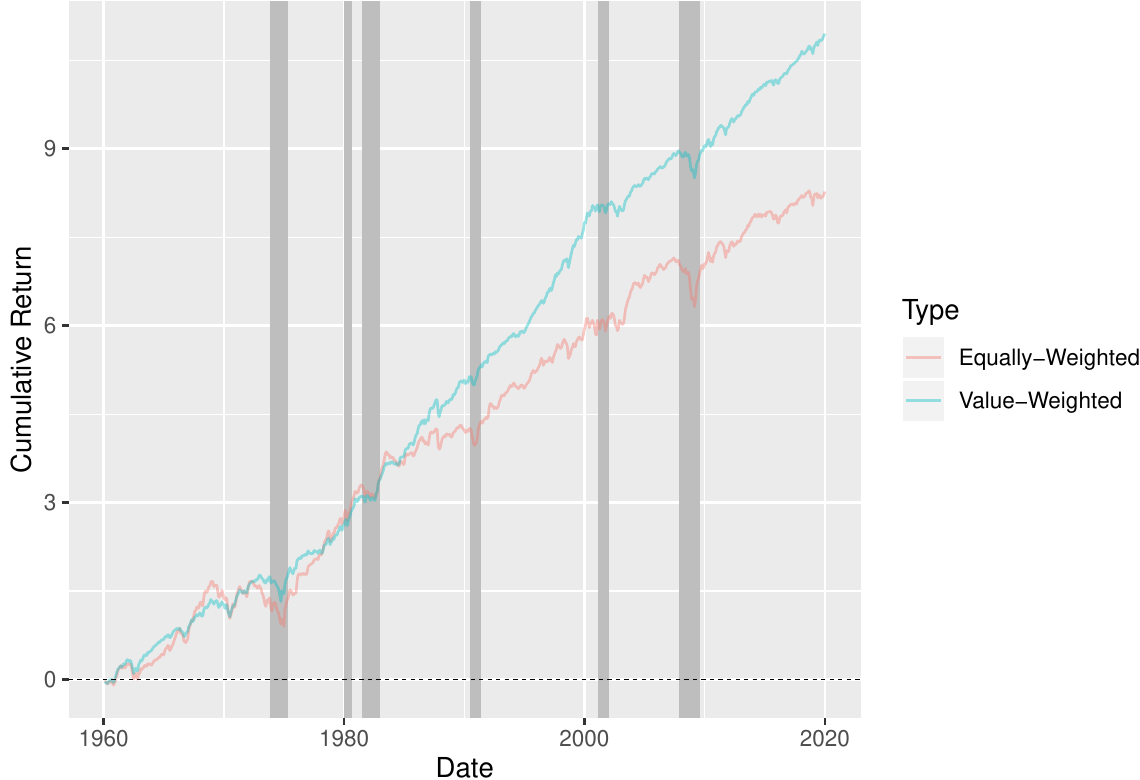
\includegraphics[width=1\linewidth]{RJ-2025-017_files/figure-latex/unnamed-chunk-12-1} \end{center}

\subsubsection{Using IC to select tuning parameters}\label{using-ic-to-select-tuning-parameters}

When jointly optimizing the tuning parameter selection the same values of \(\lambda\) and \(a\) will be selected for each quantile by minimizing \eqref{eq:jointQic}. Otherwise, the optimal tuning parameters will be selected by minimizing \eqref{eq:qic} for each quantile separately. Users can specify \texttt{method="AIC"}, \texttt{method="BIC"} or \texttt{method="PBIC"} for a large \(p\) BIC proposed by \citet{qrbic}. When doing joint selection, users can also specify \texttt{weights}, \(z_b\) in \eqref{eq:jointQic}. The default is to provide an equal weight, of one, for all quantiles.

The below code selects the tuning parameters of \((\lambda,a)\) for the \texttt{qmult} model using AIC. This code will create two \texttt{qic.select} objects, \texttt{qic\_sep} and \texttt{qic\_joint}.

\begin{verbatim}
qic_sep <- qic.select(qmult,method="AIC")
qic_joint <- qic.select(qmult, method="AIC", septau=FALSE)
\end{verbatim}

Below provides the tuning parameters selected by the two different approaches. The \texttt{modelsInfo} attribute provides information on the model selected for each quantile.

\begin{verbatim}
qic_sep$modelsInfo
\end{verbatim}

\begin{verbatim}
#>      tau modelIndex     a      minQIC lambdaIndex      lambda
#>    <num>      <int> <num>       <num>       <int>       <num>
#> 1:   0.1          1     3 -0.80983835         100 0.001744156
#> 2:   0.5          3     3  0.05987224          71 0.006721156
#> 3:   0.9          5     3 -0.86499611          82 0.004029227
\end{verbatim}

\begin{verbatim}
qic_joint$modelsInfo
\end{verbatim}

\begin{verbatim}
#>          modelIndex a tau      minQIC lambdaIndex      lambda
#> tau0.1a3          1 3 0.1 -0.80983835         100 0.001744156
#> tau0.5a3          3 3 0.5  0.06799888         100 0.001744156
#> tau0.9a3          5 3 0.9 -0.86105610         100 0.001744156
\end{verbatim}

The above tables provide the following information for the models selected for each quantile.

\begin{itemize}
\item `tau`: The quantile being modeled.
\item `a`: The value of $a$ selected.
\item `minQIC`: The QIC value for the given quantile and tuning parameters.
\item `lambdaIndex`: The position in the sequence for the preceding $\lambda$ value.
\item `lambda`: The value of $\lambda$ at the minimum cross-validation error.
\end{itemize}

When defining \texttt{qic\_joint} we set \texttt{septau=FALSE}. Thus only a single pair of \((\lambda,a)\) is selected to the be the best for all nine quantiles. That is why the values of \texttt{lambda} and \texttt{a} are the same for all quantiles in \texttt{qic\_joint\$modelsInfo}, but can differ in \texttt{qic\_sep\$modelsInfo}. The coefficients can be extracted using \texttt{coef()}.

\begin{verbatim}
coef(qic_sep)
\end{verbatim}

\begin{verbatim}
#>                 tau=0.1      tau=0.5      tau=0.9
#> intercept  0.0238504916 -0.024276359 -0.045586339
#> lgdp2     -0.0267825117 -0.024713637 -0.034210392
#> mse2       0.0129219159  0.010444821  0.017737529
#> fse2       0.0008487373  0.000000000 -0.004439600
#> fhe2      -0.0186593726  0.000000000  0.000000000
#> mhe2       0.0081453667  0.000000000  0.000000000
#> lexp2      0.0487678850  0.057746988  0.085483398
#> lintr2    -0.0010966058 -0.001761961 -0.002291657
#> gedy2     -0.3527018635 -0.068097230 -0.035234865
#> Iy2        0.0853432506  0.081856907  0.057654273
#> gcony2    -0.2044733845 -0.098175742 -0.084273528
#> lblakp2   -0.0226578393 -0.026987474 -0.033076575
#> pol2      -0.0282535823 -0.025880939  0.000000000
#> ttrad2     0.1155784172  0.140594440  0.225825288
\end{verbatim}

\begin{verbatim}
coef(qic_joint)
\end{verbatim}

\begin{verbatim}
#>                 tau=0.1       tau=0.5      tau=0.9
#> intercept  0.0238504916 -0.0326938848 -0.039997413
#> lgdp2     -0.0267825117 -0.0268792897 -0.034043618
#> mse2       0.0129219159  0.0108844720  0.018840828
#> fse2       0.0008487373  0.0000000000 -0.005800585
#> fhe2      -0.0186593726  0.0003025406  0.000000000
#> mhe2       0.0081453667  0.0052844922  0.002750732
#> lexp2      0.0487678850  0.0639833573  0.083730580
#> lintr2    -0.0010966058 -0.0020594254 -0.002348213
#> gedy2     -0.3527018635 -0.0471775148 -0.047890233
#> Iy2        0.0853432506  0.0797565855  0.059880455
#> gcony2    -0.2044733845 -0.0973417525 -0.088821669
#> lblakp2   -0.0226578393 -0.0264829810 -0.033128704
#> pol2      -0.0282535823 -0.0314157975  0.001284625
#> ttrad2     0.1155784172  0.1654870976  0.227607952
\end{verbatim}

\subsubsection{Predictions from models}\label{predictions-from-models}

Users can make predictions from either the \texttt{qic.select} or \texttt{rq.pen.seq} objects. Prediction from a \texttt{qic.select} object will return predictions for all quantiles modeled.

\begin{verbatim}
# creating new data using the mean of all variables
newData <- apply(barro,2,mean)[-1] #removing response
predict(qic_sep,newData)
\end{verbatim}

\begin{verbatim}
#>            tau=0.1    tau=0.5    tau=0.9
#> [1,] -0.0002466134 0.01894553 0.03922352
\end{verbatim}

The default for \texttt{predict()} for an \texttt{rq.pen.seq} object is to return predictions for all values of \(\lambda\), \(a\), and \(\tau\). For \texttt{qmult} this results in 900 predictions for one row of predictors because there are 100 \(\lambda\) values, 3 \(a\) values, and 3 quantiles being modeled.

\begin{verbatim}
allPreds <- predict(qmult,newData)
allPreds[,1:5] #Present the first five predictions
\end{verbatim}

\begin{verbatim}
#> tau0.1a3 L1 tau0.1a3 L2 tau0.1a3 L3 tau0.1a3 L4 tau0.1a3 L5 
#> -0.01338804 -0.01338804 -0.01338804 -0.01338804 -0.01338804
\end{verbatim}

Following the \texttt{coef.rq.pen.seq} code presented in the previous section, users can specify predictions from specific values of \(\lambda\), \(\tau\), or \(a\).

\begin{verbatim}
somePreds <- predict(qmult,newData, tau=c(.1,.5,.9),a=4,lambda=qmult$lambda[25])
somePreds
\end{verbatim}

\begin{verbatim}
#>          tau0.1a4   tau0.5a4   tau0.9a4
#> [1,] -0.008353503 0.01773852 0.05166048
\end{verbatim}

\subsubsection{Cross-validation for tuning parameter selection}\label{cross-validation-for-tuning-parameter-selection}

The function \texttt{rq.pen.cv()} creates an \texttt{rq.pen.seq.cv} object that can be used to select tuning parameters. Below we consider a similar model but use elastic net instead of SCAD. We set \texttt{tauWeights} to have \(z_b=\tau_b(1-\tau_b)\), which provides more weights to errors at the median and less to the more extreme quantiles.

\begin{verbatim}
set.seed(1)
tauVals <- c(.1,.5,.9)
qcv <- rq.pen.cv(x,y,tau=tauVals,a=c(.1,.5,1),penalty="ENet",
                 tauWeights = tauVals*(1-tauVals))
\end{verbatim}

The \texttt{plot()} function with an \texttt{rq.pen.seq.cv} object can create a plot of cross-validation error for a single quantile, \eqref{eq:cv1}, or across all quantiles, \eqref{eq:cv3}. The following provides a plot for cross-validation error for \(\tau=.5\) as a function of \(\lambda\) and \(a\).

\begin{verbatim}
plot(qcv,tau=.5)
\end{verbatim}

\begin{center}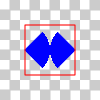
\includegraphics[width=1\linewidth]{RJ-2025-017_files/figure-latex/unnamed-chunk-20-1} \end{center}

The error bars are only provided for the sequence associated with the optimal value of \(a\), \(a=.5\) in this example. The dashed lines are only for that optimal value, too. The first dashed line is at the value of \(\lambda\) that minimizes the cross-validation error, while the second dashed line is at the value of \(\lambda\) which is one standard error above the minimum value. Users can also get a similar plot that describes how the cross-validation error across all quantiles changes with \(\lambda\) and \(a\). If a user is only interested in one quantile then the above and below plot would be identical.

\begin{verbatim}
plot(qcv,septau=FALSE)
\end{verbatim}

\begin{center}
\includegraphics[width=1\linewidth]{RJ-2025-017_files/figure-latex/unnamed-chunk-21-1} \end{center}

For an \texttt{rq.pen.seq.cv} object the \texttt{predict()} function relies on the \texttt{coef()} function. Below are four predictions using the four combinations of \texttt{septau} and \texttt{cvmin}.

\begin{verbatim}
p1 <- predict(qcv,newData)
p2 <- predict(qcv,newData, septau = FALSE)
p3 <- predict(qcv,newData, cvmin=FALSE)
p4 <- predict(qcv,newData, septau=FALSE,cvmin=FALSE)
pred <- cbind(t(p1),t(p2),t(p3),t(p4))
colnames(pred) <- c("sepMin","jointMin","sep1se","joint1se")
pred
\end{verbatim}

\begin{verbatim}
#>                 sepMin     jointMin       sep1se     joint1se
#> tau0.1a0.1 -0.00170812 -0.002409442 -0.006801621 -0.006044798
#> tau0.5a0.1  0.01895257  0.018958411  0.019494565  0.017972817
#> tau0.9a1    0.03892322  0.038575608  0.051660477  0.051154967
\end{verbatim}

The \texttt{print()} of an \texttt{rq.pen.seq.cv} object provides information about the cross-validation results.

\begin{verbatim}
qcv <- rq.pen.cv(x,y,tau=tauVals,a=c(.1,.5,1),penalty="ENet",
                 tauWeights = tauVals*(1-tauVals))
qcv
\end{verbatim}

\begin{verbatim}
#> 
#> Cross validation tuning parameter optimized for each quantile
#>      tau       minCv      lambda lambdaIndex  lambda1se lambda1seIndex     a
#>    <num>       <num>       <num>       <int>      <num>          <int> <num>
#> 1:   0.1 0.003125878 0.002005356          98 0.09308038             43   0.5
#> 2:   0.5 0.006990980 0.008095657          78 0.23056721             30   0.5
#> 3:   0.9 0.002900349 0.013193903          71 0.08680707             44   0.1
#>            cvse modelsIndex nonzero  nzse
#>           <num>       <int>   <int> <int>
#> 1: 0.0007264311           2      14     5
#> 2: 0.0014415984           5      11     3
#> 3: 0.0006872771           7      13    11
#> 
#> Cross validation tuning parameter optimized across all quantiles
#>      tau       minCv     lambda lambdaIndex lambda1se lambda1seIndex     a
#>    <num>       <num>      <num>       <int>     <num>          <int> <num>
#> 1:   0.1 0.002291483 0.01230468          72 0.3268231             25   0.1
#> 2:   0.5 0.002291483 0.01230468          72 0.3268231             25   0.1
#> 3:   0.9 0.002291483 0.01230468          72 0.3268231             25   0.1
#>            cvse modelsIndex nonzero  nzse
#>           <num>       <int>   <int> <int>
#> 1: 0.0003916137           1      14     6
#> 2: 0.0003916137           4      13    11
#> 3: 0.0003916137           7      13     4
\end{verbatim}

The printed output returns results optimized at each quantile and grouping across all quantiles.

\begin{itemize}
\item `tau`: The quantile being modeled.
\item `minCv`: The value of the minimum cross-validation error.
\item `lambda`: The value of $\lambda$ at the minimum cross-validation error.
\item `lambdaIndex`: The position in the sequence for the preceding $\lambda$ value.
\item `lambda1se`: The $\lambda$ value using the one standard error rule.
\item `a`: The optimal value of $a$ decided by the minimum cross-validation error, and the same value is used for the one standard error $\lambda$ value.
\item `cvse`: The standard error of the cross-validation error for the values of $(\lambda,a)$ that provide the smallest cross-validation error.
\item `modelsIndex`: The position of the corresponding `rq.pen.seq` object in the `$fit$models` list.
\item `nonzero`: The number of nonzero coefficients at the minimum value.
\item `nzse`: The number of nonzero coefficients at the one standard error rule.
\end{itemize}

\subsubsection{Crossing quantiles}\label{crossing-quantiles}

Crossing quantiles occurs when multiple quantiles are being modeled and predictions of a lower quantile are larger than predictions from an upper quantile. Take the following example using the Barro data set that looks at the fitted values for a model of the .1, .2 and .5 quantiles, for the 50th value in the \(\lambda\) sequence.

\begin{verbatim}
qCross <- rq.pen.cv(x,y,tau=c(.1,.2, .5))
fitCross <- predict(qCross,newx=x)
\end{verbatim}

\begin{verbatim}
#> Warning in checkCrossSep(preds, sort, object$fit$penalty): Crossing quantiles
#> at observations 17, 28, 40, 79, 94, 109, 139, 152 when using seperate
#> optimization for each lambda. Setting septau=FALSE may reduce the number of
#> crossings. In addition, using rq.gq.pen() may reduce the number of crossings.
\end{verbatim}

Warnings are provided about potential crossings at observations 17, 28, 40, 79, 94, 109, 139, and 152. Further inspection verifies this is the case as the fitted values at these observations have the .1 quantile larger than the .2 quantile. Examining these predictions verifies that is the case.

\begin{verbatim}
fitCross[c(17, 28, 40, 79, 94, 109, 139, 152),]
\end{verbatim}

\begin{verbatim}
#>                      tau0.1a1     tau0.2a1     tau0.5a1
#> Zimbabwe75       2.477067e-02  0.024519238  0.031127465
#> United_States75  1.252791e-02  0.009830172  0.014629574
#> Indonesia75      2.545159e-02  0.024898722  0.037985364
#> Gambia85        -3.663382e-03 -0.004988545  0.009901519
#> Zaire85         -3.490489e-02 -0.034921445 -0.019417390
#> United_States85 -5.850236e-05 -0.005162521  0.005242369
#> Yemen85          1.213681e-02  0.006765797  0.016998950
#> Norway85         3.488170e-02  0.034015862  0.046534611
\end{verbatim}

There is an option to sort the predictions when there are crosses. The default is not to do this because crossing quantiles can often be evidence of a misspecified model. Even when using the sort option there is a warning provided that the original predictions had crossing values.

\begin{verbatim}
fitSort <- predict(qCross, newx=x, sort=TRUE)
\end{verbatim}

\begin{verbatim}
#> Warning in checkCrossSep(preds, sort, object$fit$penalty): Quantile predictions
#> sorted at observations 17, 28, 40, 79, 94, 109, 139, 152 when using seperate
#> optimization for each lambda. Setting septau=FALSE may reduce the number of
#> crossings. In addition, using rq.gq.pen() may reduce the number of crossings.
\end{verbatim}

\begin{verbatim}
fitSort[c(17, 28, 40, 79, 94, 109, 139, 152), ]
\end{verbatim}

\begin{verbatim}
#>                     tau0.1a1      tau0.2a1     tau0.5a1
#> Zimbabwe75       0.024519238  2.477067e-02  0.031127465
#> United_States75  0.009830172  1.252791e-02  0.014629574
#> Indonesia75      0.024898722  2.545159e-02  0.037985364
#> Gambia85        -0.004988545 -3.663382e-03  0.009901519
#> Zaire85         -0.034921445 -3.490489e-02 -0.019417390
#> United_States85 -0.005162521 -5.850236e-05  0.005242369
#> Yemen85          0.006765797  1.213681e-02  0.016998950
#> Norway85         0.034015862  3.488170e-02  0.046534611
\end{verbatim}

\subsubsection{Consistent selection across quantiles}\label{consistent-selection-across-quantiles-1}

Note the output for \texttt{coefficients(qic\_sep)} and \texttt{coefficients(qic\_joint)} both show the sparsity structure changes with the quantile being modeled. We find interpreting such results to be difficult. A penalty that enforces the same sparsity structure across quantiles would avoid this issue. The following code will minimize \eqref{eq:gql}. Coefficients from the 13th entry in the \(\lambda\) sequence demonstrate that this approach provides consistency in variable selection across the quantiles. This property will hold for any value of \(\lambda\). The function \texttt{rq.gq.pen.cv()} can be used for cross-validation of this approach. The function \texttt{rq.gq.pen()} returns a \texttt{rq.pen.seq} object and thus functions such as \texttt{predict()}, \texttt{plot()}, and \texttt{qic.select()} will work as previously described.

\begin{verbatim}
qCons <- rq.gq.pen(x,y,tau=tauVals)
coefficients(qCons,lambdaIndex=13)
\end{verbatim}

\begin{verbatim}
#>                tau0.1a1      tau0.5a1     tau0.9a1
#> intercept -0.1039717886  0.0565817889  0.212830365
#> lgdp2     -0.0002948174 -0.0003086188 -0.000304075
#> mse2       0.0000000000  0.0000000000  0.000000000
#> fse2       0.0000000000  0.0000000000  0.000000000
#> fhe2       0.0000000000  0.0000000000  0.000000000
#> mhe2       0.0000000000  0.0000000000  0.000000000
#> lexp2     -0.0094731519 -0.0093673950 -0.008568437
#> lintr2     0.0000000000  0.0000000000  0.000000000
#> gedy2      0.0000000000  0.0000000000  0.000000000
#> Iy2        0.0721650464  0.0699737010  0.070700812
#> gcony2    -0.0426233067 -0.0442306488 -0.038750494
#> lblakp2   -0.0290133965 -0.0290175588 -0.028373662
#> pol2      -0.0096515098 -0.0097285059 -0.010002021
#> ttrad2     0.0000000000  0.0000000000  0.000000000
\end{verbatim}

\subsection{Group Penalty Example}\label{group-penalty-example}

The Ames Housing data contains many factor variables and is available in \CRANpkg{AmesHousing}. For simplicity of presentation, we consider only Overall\_Cond, Garage\_Type, Full\_Bath, Fireplaces, and Lot\_Config as potential predictors. Some of these are categorical predictors, and thus a group penalty can account for the group structure. For the group variables some factor levels are merged due to small number of observations in a group. For instance, we combine the groups FR2 and FR3, frontage on two or three sides, in Lot\_Config because only 14 houses are in group FR3. The function \texttt{rq.group.pen()} creates an \texttt{rq.pen.seq} object, where the models are fit with a group penalty. In the below example, we fit a model for log sale price using these predictors but do not penalize the Lot\_Config variable. For the other groups the square root of the group size is used as the group penalty factor. In addition, quantile-specific penalties of \(\tau(1-\tau)\) are used. Two \texttt{rq.pen.seq} objects are fit, one with \(q=1\), \texttt{norm=1}, and the other with \(q=2\), \texttt{norm=2}.

\begin{verbatim}
library(AmesHousing)
library(forcats)
ames <- make_ames()
ames$Overall_Cond <- fct_collapse(ames$Overall_Cond,
                                  below=c("Very_Poor","Poor","Fair","Below_Average"),
                                  above=c("Above_Average","Good","Very_Good",
                                          "Excellent", "Very_Excellent"))
ames$Garage_Type <- fct_collapse(ames$Garage_Type,
                      other=c("Basment","BuiltIn","CarPort","More_Than_Two_Types"))
ames$Lot_Config  <- fct_collapse(ames$Lot_Config, frontage=c("FR2","FR3"))

x_g <- cbind(model.matrix(~ Overall_Cond+Garage_Type+Full_Bath
                          +Fireplaces+Lot_Config,ames))[,-1]

y_g <- log(ames$Sale_Price)
g <-  c(rep(1,2),rep(2,3),3,4,rep(5,3))
gpf <- sqrt(xtabs(~g))
gpf[5] <- 0
qAmes1 <- rq.group.pen(x_g,y_g,groups=g, group.pen.factor = gpf, tau=tauVals,
                      penalty="gSCAD",norm=1,tau.penalty.factor=tauVals*(1-tauVals))
qAmes2 <- rq.group.pen(x_g,y_g,groups=g, group.pen.factor = gpf, tau=tauVals,
                      penalty="gSCAD",tau.penalty.factor=tauVals*(1-tauVals))
\end{verbatim}

The below plots present how the median coefficient estimates change with \(\lambda\).

\begin{verbatim}
plot(qAmes1,tau=.5)
\end{verbatim}

\begin{center}
\includegraphics[width=1\linewidth]{RJ-2025-017_files/figure-latex/unnamed-chunk-29-1} \end{center}

\begin{verbatim}
plot(qAmes2,tau=.5)
\end{verbatim}

\begin{center}\includegraphics[width=1\linewidth]{RJ-2025-017_files/figure-latex/unnamed-chunk-29-2} \end{center}

Two important things to note from the above two plots. First, for both models, the unpenalized coefficients for \texttt{Lot\_Config} are never set to zero. Second, the group coefficients for \texttt{qAmes2} go to zero as a group. While the grouped coefficients for \texttt{qAmes1} tend to go to zero as a group but do not have to converge to zero at the same time. For instance, for \(\tau=.5\) and using the 40th value of \(\lambda\) the garage and overall condition coefficients from \texttt{qAmes1} provide a mix of zero and non-zero coefficients. This does not occur for the default setting of \(q=2\), \texttt{norm=2}.

\begin{verbatim}
coefficients(qAmes1,tau=.5, lambdaIndex=40)
\end{verbatim}

\begin{verbatim}
#>                        tau0.5a3.7
#> intercept            11.425638982
#> Overall_CondAverage   0.005564408
#> Overall_Condabove     0.000000000
#> Garage_Typeother      0.000000000
#> Garage_TypeDetchd    -0.033878344
#> Garage_TypeNo_Garage -0.036836894
#> Full_Bath             0.346115172
#> Fireplaces            0.135504921
#> Lot_ConfigCulDSac     0.081517065
#> Lot_Configfrontage   -0.066503584
#> Lot_ConfigInside     -0.023914057
\end{verbatim}

The following plot presents how the coefficients for \texttt{Full\_Bath} change with \(\tau\) at the 40th \(\lambda\) value, where \texttt{vars=7} because \texttt{Full\_Bath} is the seventh coefficient.

\begin{verbatim}
bytau.plot(qAmes1,vars=7,lambdaIndex=40)
\end{verbatim}

\begin{center}
\includegraphics[width=1\linewidth]{RJ-2025-017_files/figure-latex/unnamed-chunk-31-1} \end{center}

The \texttt{bytau.plot()} can also be used with an \texttt{rq.pen.seq.cv} object. The below code creates an \texttt{rq.pen.seq.cv} object using the group lasso penalty.

\begin{verbatim}
qgl <- rq.group.pen.cv(x_g,y_g,g,tau=tauVals)
\end{verbatim}

The below code provides the plot for the coefficient of \texttt{GarageType\_BuiltIn} using the one standard error rule and the \(\lambda\) tuning parameter is selected to be optimal across all quantiles.

\begin{verbatim}
bytau.plot(qgl,vars=7,septau=FALSE,cvmin=FALSE)
\end{verbatim}

\begin{center}
\includegraphics[width=1\linewidth]{RJ-2025-017_files/figure-latex/unnamed-chunk-33-1} \end{center}

Other functions such as \texttt{predict()}, \texttt{coef()} and \texttt{qic.select()} work the same for a group penalty method as they do for an individual penalty, presented in the Barro data set example. The \texttt{rq.pen()}, \texttt{rq.group.pen()}, and \texttt{rq.gq.pen()} functions return \texttt{rq.pen.seq} objects. While, the \texttt{rq.pen.cv()}, \texttt{rq.group.pen.cv()} and \texttt{rq.gq.pen.cv()} functions return \texttt{rq.pen.seq.cv} objects.

\section{Simulations}\label{simulations}

Alternative packages for convex penalized quantile regression that were discussed earlier are \CRANpkg{quantreg}, \CRANpkg{conquer}, \CRANpkg{hrqglas}, and \CRANpkg{hqreg}. The only one of these four that is not used by \CRANpkg{rqPen} is \CRANpkg{conquer}. In this section two simulations settings are presented to compare the speed and quality of the solution found by \CRANpkg{conquer} and \CRANpkg{rqPen} for the lasso and group lasso penalties. The maximum number of iterations for the algorithms are set to 5000 and the tolerance for convergence was set to .001. Otherwise the default options for both packages are used. Simulations were run on a Dell Latitude 7410 laptop with an Intel Core i7 vPRO processor.

\subsection{Simulations for lasso penalty}\label{simulations-for-lasso-penalty}

Let \({\bf x}_i \sim N({\bf 0}, {\bf I}_p)\) the responses are generated from a model of,\\
\begin{equation}
y_i = {\bf x}_i^\top \boldsymbol \beta^* + \epsilon_i,
\label{eq:dgp}
\end{equation}
where \(\boldsymbol \beta^*=(\tilde{\boldsymbol \beta},\mathbf{0}_{p-10})^\top\), \(\epsilon_i \sim N(0,1)\), and the errors are independent. The entries of \(\tilde{\boldsymbol \beta}\) are generated from a standard normal distribution in each simulation. Data was generated fifty times for each combination of \(n \in \{200,2000,20000\}\) and \(p \in \{30,100,300\}\). The methods were fit for 50 \(\lambda\) values equally spaced from .05 to .25. For all methods we model \(\tau=.5\).

Three algorithms are considered, \texttt{rq.pen()} with \texttt{alg="br"} and \texttt{alg="huber"}, and \texttt{conquer.reg()}. In each simulation the time it took for the algorithms to run and the value of the objective functions at the 50 different \(\lambda\) values were recorded. Using \texttt{rq.pen(alg="br")}, which relies on \CRANpkg{quantreg}, was dramatically slower than the other approaches. Results, that are consistent with the literature when comparing a penalized approximation approach to commonly used linear programming algorithms \citep{huber_cd, highdConv}. Thus we focus on the speed differences between the Huber approximation in \CRANpkg{rqPen} and the convolution smoothing approach of \CRANpkg{conquer}. Figure \ref{fig:lassoSpeedCompare} presents a comparison of the base 10 log time of the two approaches for different values of \(n\) and \(p\), which demonstrates that the Huber approximation approach in \CRANpkg{rqPen}, which relies on \CRANpkg{hqreg}, is consistently faster. To compare the accuracy of the algorithms, we evaluate a ratio of the objective function, using quantile loss, at the solution to the objective function from the BR algorithm. The BR approach does not replace the quantile loss with an approximation and thus this ratio is always greater than or equal to one for both alternative approaches. Figure \ref{fig:lassoObjCompare} provides the ratios for different values of \(n\) and \(p\). Note, the ratios also would depend on \(\lambda\), but that information is not included in the figure for ease of presentation. Both approaches are providing minimized objective values very similar to the exact approach, with the Huber approximation approach tending to be a little closer.

\begin{figure}

{\centering \includegraphics[width=1\linewidth]{RJ-2025-017_files/figure-latex/lassoSpeedCompare-1} 

}

\caption{Log time in seconds of lasso quantile regression using conquer and the Huber approximation in rqPen.}\label{fig:lassoSpeedCompare}
\end{figure}

\begin{figure}

{\centering \includegraphics[width=1\linewidth]{RJ-2025-017_files/figure-latex/lassoObjCompare-1} 

}

\caption{Ratio of quantile regression lasso objective function at the rqPen-huber and conquer solutions, where rqPen-br is the baseline.}\label{fig:lassoObjCompare}
\end{figure}

\subsection{Simulations for group lasso penalty}\label{simulations-for-group-lasso-penalty}

For group lasso let \(\mathbf{x}_{ij}=(x_{ij1},x_{ij2})^\top\), where \(P(x_{ij1}=1)=P(x_{ij2}=1)=1/3\) and these are disjoint events. That is it represents a single observation of a multinomial random variable with 3 categories and equal probability of belonging to any of the three categories. Let \(\mathbf{x}_i = (\mathbf{x}_{i1},\ldots,\mathbf{x}_{ig})^\top\), where the predictors are independent of each other. The data generating mechanism for \(y\) is the same as \eqref{eq:dgp}. Again, data was generated fifty times for each combination of \(n \in \{200,2000,20000\}\) and \(g \in \{15,50,150\}\). The methods were fit for 50 \(\lambda\) equally spaced values from .05 to .001. Again, for all methods we model \(\tau=.5\).

The group lasso methods implemented in rqPen, using \texttt{rq.group.pen()}, and conquer, using \texttt{conquer.reg(penalty="group",...)} are compared in these simulations. Both approaches replace the quantile loss function with a smooth approximation. When the quantile loss is used, the optimization problem is a second order cone programming problem that can be solved using convex optimization software. See \citet{SherwoodLi2022} for a comparison of the Huber approximation approach and using \CRANpkg{Rmosek} for quantile regression with a group lasso penalty. To compare the two methods time and a ratio of the rqPen and conquer penalized objective functions evaluated at the solutions. Figure \ref{fig:lassoSpeedCompareGroup} and \ref{fig:lassoObjCompareGroup} present the time and objective function results, respectively. While, \CRANpkg{rqPen} tends to find a solution that provides a smaller value at the objective function, the results from \CRANpkg{conquer} are noticeably faster. Note, the implementation of group lasso in \CRANpkg{rqPen} relies on \CRANpkg{hrqglas}.

\begin{figure}

{\centering \includegraphics[width=1\linewidth]{RJ-2025-017_files/figure-latex/lassoSpeedCompareGroup-1} 

}

\caption{Log time in seconds of group lasso quantile regression using conquer and the Huber approximation in rqPen.}\label{fig:lassoSpeedCompareGroup}
\end{figure}

\begin{figure}

{\centering \includegraphics[width=1\linewidth]{RJ-2025-017_files/figure-latex/lassoObjCompareGroup-1} 

}

\caption{Ratio of quantile regression group lasso objective function at the rqPen and conquer group lasso solutions.}\label{fig:lassoObjCompareGroup}
\end{figure}

\section{Summary}\label{summary}

The \CRANpkg{rqPen} package provides a penalized approach to estimating quantile regression models. The package supports the elastic-net, adaptive lasso, SCAD, and MCP penalty functions. For group predictors there are group penalty versions of the lasso, adaptive lasso, SCAD, and MCP penalties. In addition, users can use a group quantile penalty that ensures consistent variable selection across the quantiles. The package is available on CRAN.

Research in penalized quantile regression, and more generally quantile regression with large data sets, is an active area of research. The package currently does not include some recent innovations in the field. Censored quantile regression is a useful tool for survival analysis and an active area of research. \citet{hdCensQR} present a penalized quantile regression approach for estimating an interval of quantiles for censored data. While, \citet{effCenQR} provides a unifying approach to estimation and inference for censored quantile regression that possibly could be extended to penalized settings. Another interesting work that provides a framework that could possibly be extended to penalized quantile regression is \citet{qrDist}, which proposes a method for estimating quantile regression that splits up initial analysis across multiple computers and then combines the estimates. A challenge here would be dealing with the different sparsity patterns that could arise on the different machines. Inference for penalized methods has also been an active area of research. Recently, \citet{validQRInf} propose an approach where they do not approximate the quantile loss function and \citet{ciHypHDQR} provide an approach for when the loss function is approximated with a smoothing function. Quantiles are more easily understood when the response is continuous. For users interested in estimating conditional quantiles for count data, one easy solution is to jitter the response \citep{quantileCount}. All of these works suggest that there is a variety of existing work that could be developed into useful software and plenty of work to be done in the future.

\bibliography{RJreferences.bib}

\address{%
Ben Sherwood\\
University of Kansas\\%
School of Business\\ Lawrence, KS\\
%
%
%
\href{mailto:ben.sherwood@ku.edu}{\nolinkurl{ben.sherwood@ku.edu}}%
}

\address{%
Shaobo Li\\
University of Kansas\\%
School of Business\\ Lawrence, KS\\
%
%
%
\href{mailto:shaobo.li@ku.edu}{\nolinkurl{shaobo.li@ku.edu}}%
}

\address{%
Adam Maidman\\
University of Minnesota\\%
School of Statistics\\ Minneapolis, MN\\
%
%
%
\href{mailto:abmaidman@gmail.com}{\nolinkurl{abmaidman@gmail.com}}%
}

\end{article}


\end{document}
